\documentclass{standalone}
\usepackage{tikz}

\begin{document}
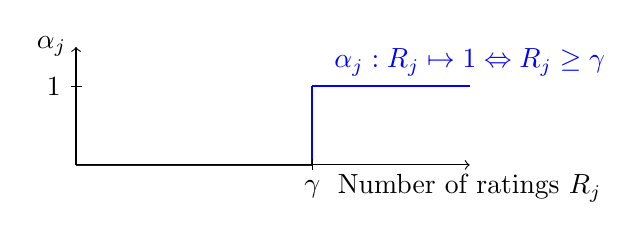
\begin{tikzpicture}
% Draw the log-normal distribution curve
\draw[blue,smooth,thick] plot[id=f1,domain=0:3,samples=50]
({\x,0});
\draw[blue,thick] (3,0) -- (3,1);
\draw[blue,smooth,thick] plot[id=f1,domain=3:5,samples=50]
({\x,1}) node[above] {$\alpha_j : R_j \mapsto 1 \Leftrightarrow R_j \geq \gamma$};
%({\x,{1/(1+exp(-3*(\x-3)))}}) node[above] {$\alpha_j : R_j \mapsto 1/(1 + \exp(-\beta(R_j - \gamma)))$};
% Draw the x-axis
\draw[->,black] (0,0) -- (5,0) node[below] {Number of ratings $R_j$};
% Draw the y-axis
\draw[->,black] (0,0) -- (0,1.5) node[left] {$\alpha_j$};
\draw (3,2pt) -- ++(0,-4pt) node[below] {$\gamma$};
\draw (2pt,1) -- ++(-4pt,0) node[left] {1};
%\draw (2pt,.5) -- ++(-4pt,0) node[left] {1/2};
%\draw[dashed] (0,.5) -- (3,.5);
%\draw[dashed] (3,0) -- (3,.5);
\end{tikzpicture}
\end{document}